\documentclass{article}
\usepackage{graphicx} % Required for inserting images
\usepackage[ngerman]{babel}
\usepackage{enumitem}
\usepackage{float}
\usepackage{chngcntr}
\usepackage{glossaries}
\counterwithin{figure}{section}
\setlength\parindent{0pt}

\makeglossaries

\newglossaryentry{Attributsableitung}
{
    name=Attributsableitung,
    description={Platzhalter-Implementierung eines Glossar-Eintrags.}
}

\newglossaryentry{Verkehrsmodell}
{
    name=Verkehrsmodell,
    description={Platzhalter-Implementierung eines Glossar-Eintrags.}
}

\newglossaryentry{Discrete Choice}
{
    name=Discrete Choice,
    description={Platzhalter-Implementierung eines Glossar-Eintrags.}
}

\newglossaryentry{Projektdatei}
{
    name=Projektdatei,
    description={Kann eine CSV-Datei, Attributsableitungen, Alternativen und Nutzenfunktionen beinhalten.}
}

\newglossaryentry{Alternative}
{
    name=Alternative,
    description={Eine alternatives Verkehrsmittel.}
}

\title{Pflichtenheft \\ \large Einflussfaktoren auf die Verkehrsmittelwahl\\ -- Baukasten für Discrete Choice Modelle}
\author{Kevin Boehnke \\ \texttt{uxpkw@student.kit.edu}
\and Floriane Bresser \\ \texttt{uspvq@student.kit.edu}
\and Damian Reich \\ \texttt{uqppn@student.kit.edu}
\and Alissa Saleh \\ \texttt{unmbc@student.kit.edu}
\and Michael Schur \\ \texttt{ufkmz@student.kit.edu}}
\date{24. Mai 2023}

\begin{document}
\clearpage\maketitle\thispagestyle{empty}
\newpage
\clearpage\tableofcontents\thispagestyle{empty}
\newpage
\pagenumbering{arabic}

\section{Einleitung}

Im Alltag existieren viele Einflussfaktoren auf die Verkehrsmittelwahl, wie die demographische Entwicklung, Infrastrukturmaßnahmen, Veränderungen in Siedlungsstrukturen, Steuerungsmaßnahmen, veränderte Energiepreise oder Maßnahmen des Mobility Pricings. Zur Schaffung einer quantitativen Basis, die verkehrsplanerische, betriebswirtschaftliche und politische Entscheidungen unterstützt, werden Verkehrsmodelle eingesetzt.\newline

Ein Verkehrsnachfragemodell ist die Diskrete Entscheidungsmodellierung. In diesem werden jeder Wahlmöglichkeit Aufteilungs- und Nutzenfunktionen zugewiesen, die auf Parametern beruhen. Die Parameter werden mittels der Maximum-Likelihood-Schätzung aus Umfrageergebnissen geschätzt, in denen die Befragten Aussagen über ihr Verhalten bei der Verkehrsmittelwahl machen. Ebenfalls können Parameter mittels der Stated Choice Methode geschätzt werden. Diese basiert auf hypothetischen Entscheidungssituationen zwischen Alternativen mit zugewiesenen Attributen. Eine Stated Choice Parameterschätzung beginnt mit Entscheidungen über die Alternativen und ihrer Attribute und der Erwartung möglicher Nutzenfunktionen zur Optimierung des Designs des Stated Choice Experiment. Anschließend wird das Design implementiert und die Befragung umgesetzt. Im letzten Schritt soll das Aufbereiten der Daten und Abschätzen der Parameter erfolgen.\newline

Der Baukasten übernimmt dabei das Einlesen und Aufbereiten der Daten und ermöglicht durch Berechnungen im Rahmen der Modelle eine Schätzung und Visualisierung der Parameter. Durch die Möglichkeit individuell definierter Funktionen soll das Produkt diesen Ablauf vereinfachen und eine automatisierte Parameterschätzung sowie die Visualisierung der Modelle ermöglichen. 

\newpage
\section{Zielbestimmung}
Das Produkt unterstützt die Verkehrsingenieure dabei, Discrete Choice Modelle in der Verkehrsmittelwahl zu erstellen, modifizieren und visualisieren.
\subsection{Musskriterien}
\begin{itemize}
    \item[\textbf{/MK1/}] Der Nutzer kann Erhebungsdaten im CSV-Format importieren.
    \item[\textbf{/MK2/}] Der Nutzer kann Tabellen durch Attributsableitungen erweitern.
    \subitem Folgende Möglichkeiten stehen dem Nutzer zur Verfügung:
    \begin{itemize}[leftmargin=.7in]
        \item[\textbf{/MK2.1/}] Intervalle
        \item[\textbf{/MK2.2/}] Gruppen
        \item[\textbf{/MK2.3/}] Logische Ausdrücke
        \item[\textbf{/MK2.4/}] Vergleiche
    \end{itemize}
    \item[\textbf{/MK3/}] Der Nutzer kann Alternativen hinzufügen und löschen.
    \item[\textbf{/MK4/}] Der Nutzer kann für jede Alternative eine Nutzenfunktion definieren und ändern.
    \begin{itemize}[leftmargin=.7in]
        \item[\textbf{/MK4.1/}] Der Nutzer kann Linearkombinationen für die Nutzenfunktion verwenden.
    \end{itemize}
    \item[\textbf{/MK5/}] Der Nutzer kann die Parameter und Signifikanz aus gegebener Eingabe und Modellstruktur berechnen lassen.
    \item[\textbf{/MK6/}] Das Programm bietet eine Schnittstelle für andere Bibliotheken zur Parameterschätzung und Signifikanzgewinnung. 
    \begin{itemize}
        \item Es wird standardmäßig das Python Paket \textit{Biogeme} verwendet.
    \end{itemize}
    \item[\textbf{/MK7/}] Das Programm visualisiert die gewonnenen Parameter und Signifikanzniveaus.
    \item[\textbf{/MK8/}] Der Nutzer kann die Ergebnisse der Berechnung und die Visualisierung exportieren.
    \item[\textbf{/MK9/}] Das Programm bietet eine Schnittstelle um die Parameteraufteilung zu erweitern oder einzuteilen anhand der Signifikanzniveaus.
    \item[\textbf{/MK10/}] Der Nutzer kann ein Projekt als Projektdatei speichern und laden.
\end{itemize}

\subsection{Wunschkriterien}
\begin{itemize}
    \item[\textbf{/WK1/}] Das Programm unterstützt arbiträre Funktionen in der Attributaufbereitung.
    \item[\textbf{/WK2/}] Die vom Nutzer definierten Funktionen können gespeichert werden.
    \item[\textbf{/WK3/}] Der Nutzer wird bei der Programmführung durch folgende Funktionen von der Software unterstützt:
    \begin{itemize}[leftmargin=.7in]
        \item[\textbf{/WK3.1/}] Autovervollständigung
        \item[\textbf{/WK3.2/}] Typhinweise
        \item[\textbf{/WK3.3/}] Fehlerunterbindung
    \end{itemize}

    \item[\textbf{/WK4/}] Die Nutzenfunktionen im Modell-Aufbau können wie folgt verschachtelt werden:
    \begin{itemize}[leftmargin=.7in]
        \item[\textbf{/WK4.1/}] Arithmetik: $\beta \cdot (T + (\beta_2 \cdot X_2 \cdots))$
        \item[\textbf{/WK4.2/}] Exponentialfunktionen: $\log(T)$, ${\rm e}^T$
        \item[\textbf{/WK4.3/}] Potenzen: $\beta \cdot X^3$
    \end{itemize}
    \item[\textbf{/WK5/}] Das Programm kann um andere Modell-Strukturen, wie beispielsweise Nested Logit, erweitert werden.
    \item[\textbf{/WK6/}] Der Nutzer kann die Schwellwerte für die Signifikanz selber konfigurieren.
    \begin{itemize}
        \item Beispiel bei Apollo: $|T-Ratio | > 1.95$, $|Robust T-Ratio | > 1.95$
    \end{itemize}    
    \item[\textbf{/WK7/}] Es existiert ein vollwertiger Algorithmus zur Bestimmung von Signifikanzgruppen und Aufteilungen.
    \item[\textbf{/WK8/}] Die Anwendung kann auf einer Workstation, Windows Server, 8 Kerne (16 logische Kerne) ausgeführt werden. 
    
\end{itemize}
\subsection{Abgrenzungskriterien}

\newpage
\section{Produkteinsatz}
\subsection{Anwendungsbereiche}
Der vorgesehene Anwendungsbereich ist die Verkehrsmodellierung aus Befragungsdaten im Bereich der Verkehrswissenschaften. Die Anwendung eignet sich zur Modellierung für eine Prognose als Basis für verkehrsplanerische, betriebswirtschaftliche und politische Entscheidungen, ebenso wie als Verwendung in der Recherche.

\subsection{Zielgruppen}
Das Produkt richtet sich an Verkehrsingenieure und Verkehrswissenschaftler. Zur Verwendung sind keine Vorkenntnisse im Bereich Informatik notwendig. Ebenfalls wird eine Opensource Veröffentlichung angestrebt, die weitere Nutzer ermöglicht.
  
\subsection{Betriebsbedingungen}
Der Baukasten wird als Desktopanwendung konzipiert, die in Büroumgebung ausgeführt wird. Übliche Bestriebsbedingungen sind die Nutzung zu standard Arbeitszeiten. Es ist keine Beobachtung während der Ausführung notwendig, unbeaufsichtigter Betrieb wird unterstützt und die Ausführung kann unterbrochen und zu späteren Zeitpunkten fortgeführt werden. Zur Ausführung der Anwendung wird keine Internetverwendung benötigt.
Der Baukasten ist für Laptops mit den Mindestanforderungen 8 Gb RAM, i5 (4 Kerne, 8 log.) und Windows 10/11 verfügbar. Ebenfalls kann die Anwendung auf der Workstation, Windows Server, 8 Kerne (16 log.) ausgeführt werden.
\newpage

\section{Produktumgebung}
\subsection{Software}
\begin{itemize}
    \item Die Software wird in Python geschrieben.
    \item Betriebssystem: Windows 10 oder Windows 11
    \item Die Software wird als Open Source veröffentlicht und erweiterbar sein.
\end{itemize}
\subsection{Hardware}
\begin{itemize}
    \item Das Produkt ist eine Desktopanwendung.
    \begin{itemize}
        \item Mindestanforderung: Laptop, 8GB RAM, Intel Core i5 (4 Kerne, 8 logische Kerne)
        \item \textit{WK}: Workstation, Windows Server, 8 Kerne (16 logische Kerne)
    \end{itemize}
\end{itemize}
\subsection{Schnittstelle}
\begin{itemize}
    \item Die Software nimmt Dateien im CSV-Format entgegen.
    \item \textit{WK}: Die Anwendung soll über eine Schnittstelle andere Bibliotheken zur Parameterschätzung einbinden können.
    \begin{itemize}
        \item beispielsweise das \textit{Apollo Package}
    \end{itemize}
\end{itemize}
\newpage

\section{Produktfunktionen}
\subsection{Funktionsübersicht}
Im Folgenden ist eine Übersicht der Produktfunktionen.
\begin{figure}[H]%
  \centering
  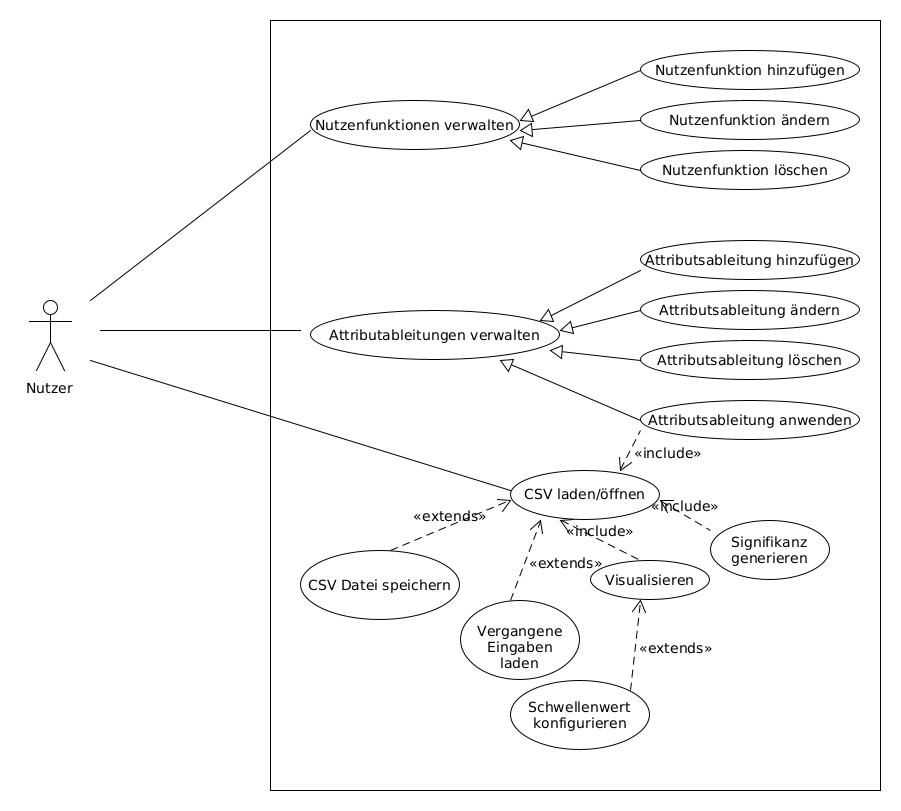
\includegraphics[width=15cm]{use case4.jpg}
  \caption{Use Case Diagramm}
\end{figure} 
\newpage
\textbf{/F10/} Erhebungsdaten lesen \\
\textbf{/F11/} CSV Datei speichern \\
\textbf{/F12/} Vorherige Eingaben laden \\
\textbf{/F15/} Attributsableitungen hinzufügen \\
\textbf{/F16/} Attributsableitungen ändern \\
\textbf{/F17/} Attributsableitungen löschen \\
\textbf{/F18/} Attributsableitungen anwenden \\
\textbf{/F20/} Nutzenfunktionen eingeben \\
\textbf{/F21/} Nutzenfunktionen ändern \\
\textbf {/F22/} Nutzenfunktionen löschen \\
\textbf{/F25/} Signifikanzgenerierung \\
\textbf{/F30/} Visualisieren \\
\textbf{/F35/} Schwellwerte konfigurieren
%\newpage
\\[0.5in]
\subsubsection*{/F10/ Erhebungsdaten lesen}
\underline {Ziel}:   Bereits existiernde CSV Datei öffnen, welche die nötigen Erhebungsdaten beinhaltet. \\
\underline{Vorbedingung}: keine\\
\underline{Beschreibung}: Nutzer öffnet CSV Datei.
\subsubsection*{/F11/ CSV Datei speichern}
\underline{Ziel}: Hinzugefügte Spalten in der CSV Datei speichern. \\
\underline{Vorbedingung}: keine \\
\underline{Beschreibung}: Die durch Attributsableitungen entstandene Spalten werden in der (selben? neuen?) CSV Datei gespeichert.
\subsubsection*{/F12/ Vorherige Eingaben laden}
\underline{Ziel}: Bereits eingegebene Funktionen und Nutzenfunktionen laden. \\
\underline{Vorbedingung}: CSV Datei muss geöffnet sein; Vergangene Eingaben müssen existieren. \\
\underline{Beschreibung}: Eingaben werden geladen.
\subsubsection*{/F15/ Attributsableitungen hinzufügen}
\underline{Ziel}: Neue Attributsableitungen definieren. \\
\underline{Vorbedingung}: keine \\
\underline{Beschreibung}: Nutzer gibt Funktion an. Wenn die Eingabe syntaktisch korrekt ist, wird sie hinzugefügt.
\subsubsection*{/F16/ Attributsableitungen ändern}
\underline{Ziel}: Bereits existierende Attributsableitungen ändern. \\
\underline{Vorbedingung}: Existenz der Funktion, die geändert werden soll  \\
\underline{Beschreibung}: Die Funktion wird geändert, wenn die neue Eingabe syntaktisch korrekt ist.
\subsubsection*{/F17/ Attributsableitungen löschen}
\underline{Ziel}: Erfolgreiche Löschung einer Attributsableitung. \\
\underline{Vorbedingung}: Existenz der Funktion, die gelöscht werden soll.\\
\underline{Beschreibung}: Nutzer löscht die Funktion.
\subsubsection*{/F18/ Attributsableitungen anwenden}
\underline{Ziel}: Eingegebene Attributsableitungen anwenden. \\
\underline{Vorbedingung}: Attributsableitungen müssen vorher existieren; CSV Datei muss geöffnet sein. \\
\underline{Beschreibung}: Durch die Anwendung werden neue Spalten in der CSV Datei entstehen.
\subsubsection*{/F20/ Nutzenfunktionen einfügen}
\underline{Ziel}: Nutzenfunktionen für Alternativen definieren. \\
\underline{Vorbedingung}: keine \\
\underline{Beschreibung}: Nutzer gibt die Nutzenfunktion ein. Sie soll eine Linearkombination sein. Eingabe wird automatisch gespeichert ?? \\
\subsubsection*{/F21/ Nutzenfunktionen ändern}
\underline{Ziel}: Nutzenfunktionen ändern.\\
\underline{Vorbedingung}: Die zu ändernde Nutzenfunktion muss existieren bzw. vorher eingegeben werden. \\
\underline{Beschreibung}: Nutzer ändert die bereits existierende Nutzenfunktion. Wenn die Änderungen korrekt sind werden sie umgesetzt.
\subsubsection*{/F22/ Nutzenfunktionen löschen}
\underline{Ziel}: Nutzenfunktionen endgültig löschen.\\
\underline{Vorbedingung}: Die zu löschende Nutzenfunktion muss existieren. \\
\underline{Beschreibung}: Nutzer löscht die Nutzenfunktion.
\subsubsection*{/F25/ Signifikanzgenerierung}
\underline{Ziel}: Signifikanz und die Parameter bestimmen. \\
\underline{Vorbedingung}: CSV Datei muss geöffnet sein; Nutzenfunktionen müssen schon definiert sein. \\
\underline{Beschreibung}: Nutzer gibt die Anweisung, Signifikanz zu bestimmen. Diese erfolgt automatisch mit Bestimmung der Parameter durch R Biblothek Apollo.
\subsubsection*{/F30/ Visualisierung}
\underline{Ziel}: Ergebnisse der Signifikanz anschaulich machen. \\
\underline{Vorbedingungen}: CSV Datei muss geöffnet sein; Signifikanz muss vorher berechnet werden. \\
\underline{Beschreibung}: Parameterwerte und Signifikanz werden gezeigt. Nicht signifikante Parameter werden hervorgehoben.
\subsubsection*{/F35/ Schwellwerte konfigurieren}
\underline{Ziel}: Schwellwert ändern; Bestimmt welche Parameter hervorgehoben werden. \\
\underline{Vorbedingungen}: CSV Datei muss geöffnet sein; Visualisierung muss vorher betätigt werden. \\
\underline{Beschreibung}: Nutzer ändert den Schwellwert.


\section{Produktdaten}
\subsection{Projektdaten}
\subsubsection*{/D10/ Rohdaten}
\subsubsection*{/D20/ Ableitungen}
\subsubsection*{/D30/ Signifikanzen}
\subsubsection*{/D40/ Parameter}
\subsubsection*{/D50/ Verwendete Funktionen}
\subsection{Nutzenfunktionen}
\subsubsection*{/D60/ Nutzenfunktion}
\subsection{Attributableitungen}
\subsubsection*{/D70/ Ableitungsfunktion}

\section{Produktleistungen}

\section{Benutzerschnittstelle}
\begin{figure}[H]%
  \centering
  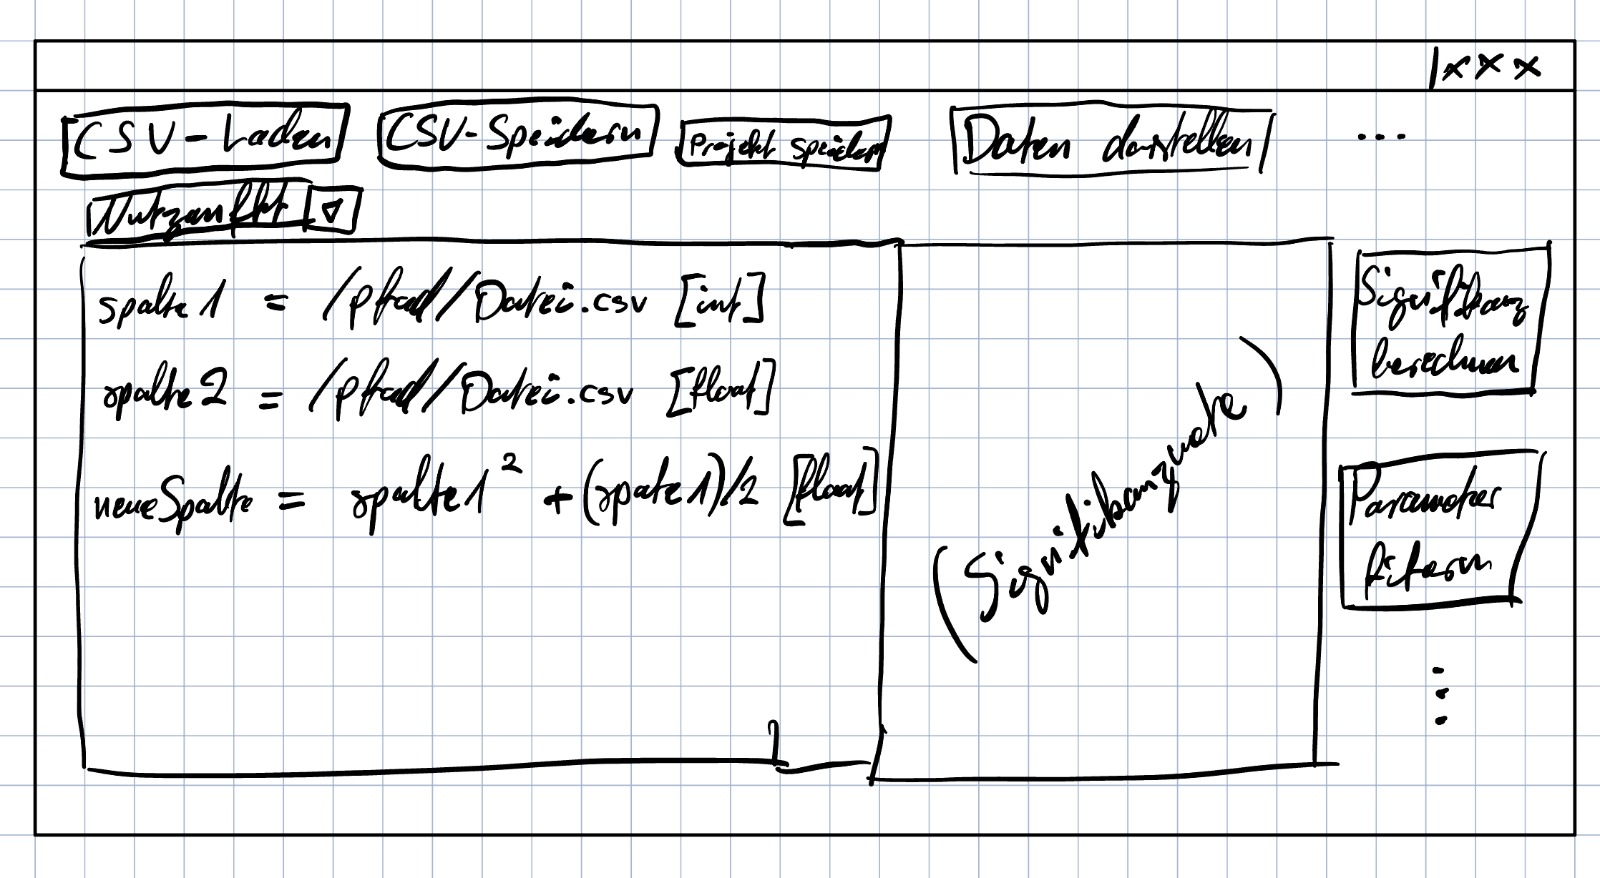
\includegraphics[width=12cm]{gui.jpeg}
  \caption{GUI Entwurf}
\end{figure}


\section{Globale Testfälle}

\section{Qualitätsbestimmung}

\begin{table}[H]
\begin{tabular}{lllll}
\hline
\textbf{Produktqualität} & sehr gut & gut & normal & nicht relevant \\ \hline
\textbf{Funktionalität}  &          &     &        &                \\
Angemessenheit           &          & X   &        &                \\
Richtigkeit              & X        &     &        &                \\
Interoperabilität        &          &     & X      &                \\
Ordnungsmäßigkeit        &          &     &        & X              \\
Sicherheit               &          &     &        & X              \\
\textbf{Zuverlässigkeit} &          &     &        &                \\
Reife                    &          &     & X      &                \\
Fehlertoleranz           & X        &     &        &                \\
Wiederherstellbarkeit    &          & X   &        &                \\
\textbf{Benutzbarkeit}   &          &     &        &                \\
Verständlichkeit         &          & X   &        &                \\
Erlernbarkeit            &          & X   &        &                \\
Bedienbarkeit            & X        &     &        &                \\
\textbf{Effizienz}       &          &     &        &                \\
Zeitverhalten            &          & X   &        &                \\
Verbrauchsverhalten      &          & X   &        &               
\end{tabular}
\end{table}

\clearpage

\glsaddall
\printglossary[%nonumberlist
]

\end{document}